\begin{DoxyWarning}{Warning}
This code is under development and has not been properly benchmarked. Feel free to use it, but be warned that it is distributed W\-I\-T\-H\-O\-U\-T A\-N\-Y W\-A\-R\-R\-A\-N\-T\-Y. Please, contact Juan Rodriguez-\/\-Gonzalez (\href{mailto:jrglez@umd.edu}{\tt jrglez@umd.\-edu}) if you make any significant modifications to this code.
\end{DoxyWarning}
\hypertarget{index_intro}{}\section{Introduction}\label{index_intro}
This code simulates the deformation of a viscoelastic medium in presence of a discrete fault under the anti-\/plane shear approximation. Under this assumption there is no displacement in the modeled plane $(u_{x}=u_{y}=0)$ and there is no spatial variation in the direction perpendicular to the modeled plane $(\partial z=0)$. We solve the equilibrium equation for an elastic medium in with an isotropic constitutive relationship in which the elastic strain is relaxed by viscous creep. Under this conditions, the right-\/hand side depends on the displacement values from the previous time step.\hypertarget{index_equations}{}\subsection{Viscoelastic approximation}\label{index_equations}
We solve the equation of equilibrium for stress in a continuum medium\-:

\[\partial_{i} \sigma = f^g_j \]

where $i$ and $j$ run from 1 to 3 and designate spatial coordinate, $\sigma$ is the stress tensor and $\boldsymbol{f^g}$ is the total external force, in this case, only the gravitational force $f^g_j=f^g_j=\rho g \left(1-\alpha T \right) \delta_{iy}$. We assume a linear maxwel model in which the total strain $ \varepsilon $ is the sum of the elastic strain $ \varepsilon^e $ and the viscous strain $ \varepsilon^v $\-:

\[ \varepsilon_{ij} = \varepsilon^e_{ij} + \varepsilon^v_{ij} + \varepsilon^0_{ij} \]

where $ \varepsilon^0 $ is the initial strain. We will use a semi-\/elastic approach \cite{zienkiewicz_cormeau_74} \cite{yamasaki_houseman_12} for which we assume a constitutive relation between stress and elastic strain\-:

\[ \sigma_{ij} = C_{ijkl} \varepsilon_{kl} + \sigma^0_{ij}\]

where $ C $ is the elastic stiffness tensor and $ \sigma^0 $ is the initial stress. This can be interpreted as the stress being relaxed by viscous creep\-:

\[ \sigma_{ij} = C_{ijkl} \left( \varepsilon_{kl} - \varepsilon^v_{kl} -\varepsilon^0_{kl} \right) + \sigma^0_{ij} \]

In an isotropic medium\-:

\[ \sigma_{ij} = \lambda \left( \epsilon_{kk} - \epsilon^0_{kk} \right) \delta_{ij} + 2\mu \left( \varepsilon_{ij} - \varepsilon^v_{ij} - \varepsilon^0_{ij} \right) + \sigma^0_{ij} \]

where $ \lambda $ is the first Lamé parameter and $\mu$ is the shear modulus. The strain can be expressed in terms of the displacement $ u_i $\-:

\[ \varepsilon_{ij} = \frac{1}{2} \left( \partial_j u_i + \partial_i u_j \right) \]

The viscous strain rate $ \dot \varepsilon^v $ depends on the stress tensor\-:

\[ \dot \varepsilon^v_{ij} = \beta_{ij}(\sigma) \]

where $ \beta $ are given functions. A relationship to link the viscous strain rate and the elastic strain is given in the next section.

We can now use this in the momentum equation and we have\-:

\[ \partial_i \left( \lambda \varepsilon_{kk} \delta_{ij} + 2 \mu \varepsilon_{ij} \right) = f_j + f^v_j \]

where

\[ f_j = f^g_j + \partial_i \left( \lambda \varepsilon^0_{kk}\delta_{ij} + 2 \mu \varepsilon^0_{ij} - \sigma^0_{ij} \right) \]

This equation is very similar to the elasticity equation but with an internal force due to the viscous coupling\-:

\[ f^v_j = \partial_i \left( 2 \mu \varepsilon^v_{ij} \right) \]\hypertarget{index_num_approach}{}\subsection{Numerical approach}\label{index_num_approach}
To use a semi-\/elastic approach we need to manipulate the constitutive equation to find a relation between viscous and elastic strains. To achieve this, the first step is to express the viscous strain in terms of the viscous strain rate. We replace the strain rate by the forward derivative\-:

\[ \dot \varepsilon^v(t_n) = \frac{\varepsilon^v(t_{n+1}) - \varepsilon^v(t_n)}{\Delta t_n} \]

where the subscripts $ n $ and $ n+1 $ indicate the current and future time steps and $ \Delta t_{n+1} = t_{n+1} - t_n $ is the time step increment. Therefore, we can write the viscous strain at a given time step as\-:

\[ \varepsilon^v(t_{n+1}) = \varepsilon^v(t_{n}) + \Delta t_{n+1} \dot \varepsilon(t_{n}) \]

Following \cite{yamasaki_houseman_12}, we use the following relation between viscous strain rate and elastic strain\-:

\[ \dot \varepsilon^v_{ij} = \frac{\mu}{\eta} \left( \varepsilon_{ij} - \frac {1}{3} \epsilon_{kk}\delta_{ij} \right) \]

where $ \eta $ is the viscosity. And at time step n+1 we will need to solve the equation\-:

\[ \partial_i \left( \lambda \varepsilon_{kk}(t_{n+1}) \delta_{ij} + 2 \mu \varepsilon_{ij}(t_{n+1}) \right) = f^g_j(t_{n+1}) + f^{v}_j(t_{n+1}) \]

where the internal elastic force now only depends on the strain and past viscous strain rate\-:

\[ f^{v}_j(t_{n+1}) = \partial_i \left( 2\mu \varepsilon^v_{ij}(t_{n+1}) \right) = \partial_i \left\{ 2\mu \left[\varepsilon^v_{ij}(t_n) + \frac{\mu \Delta t_{n+1}}{\eta} \left(\varepsilon_{ij}(t_n) - \frac{1}{3} \varepsilon_{kk}(t_n) \delta_{ij} \right) \right] \right\} \]

Therefore, we will follow the next scheme to solve the problem\-:
\begin{DoxyEnumerate}
\item Set initial conditions $ (n = 0) $ for the stress $\sigma(t_0) = \sigma^0$, displacement $ \boldsymbol{u}(t_0) $ and viscous strain $ \varepsilon^v(t_0) $.
\item Compute the viscous strain $ \varepsilon^v(t_{n+1}) $, which depends on $ \varepsilon(t_n) $ and $ \varepsilon^v(t_n) $.
\item Solve the momentum equation to obtain the displacement $ \varepsilon (t_{n+1}) $
\item Compute $ \sigma (t_{n+1}) $.
\item Update $ n \leftarrow n+1 $ and repeat steps 2 to 5.
\end{DoxyEnumerate}\hypertarget{index_anti_plane}{}\subsubsection{Anti-\/plane shear approximation}\label{index_anti_plane}
The equations presented until now are valid for viscoelastic problems in any dimensions. However, solving it can be computationally demanding. For certain problems it is enough to solve the equation under certain approximations. In this case we are going to model the displacement in the $x-y$ plane produced by a fault that runs parallel to the $y-z$ plane and is sliding parallel to the $z$ direction. 
\begin{DoxyImage}
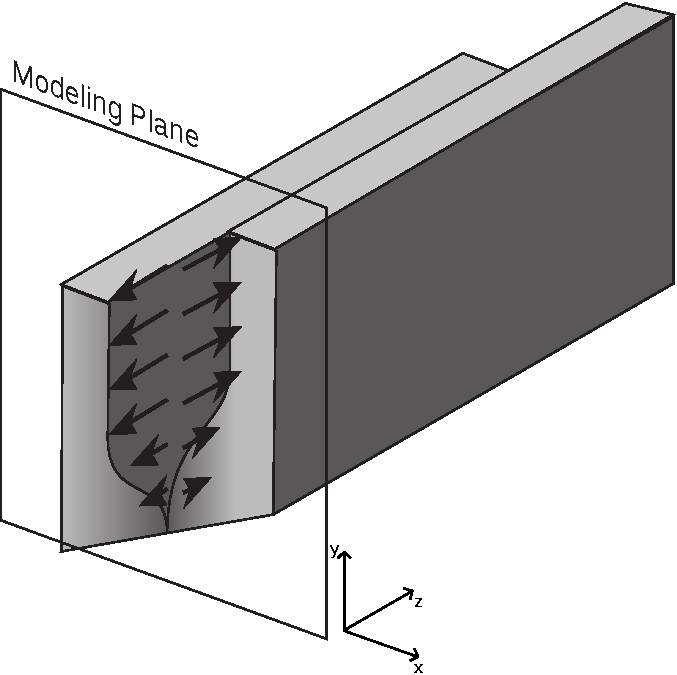
\includegraphics{aps}
\caption{Figure 1\-: Schematic representation of a fault and the modeled plane}
\end{DoxyImage}
 In this case, we can considered that displacement only occurs in the $z$ direction $ (u_{x}=u_{y}=0) $. Moreover, under this approximation no magnitude can vary along the $ z $ direction $(\frac{\partial}{\partial z}=0)$. Therefore, under this approximation $ \varepsilon_{xx} = \varepsilon_{yy} = \varepsilon_{zz} = \varepsilon_{xy} = \varepsilon_{yx}=0$, $\ast$ $ \varepsilon^v_{xx} = \varepsilon^v_{yy} = \varepsilon^v_{zz} = \varepsilon^v_{xy} = \varepsilon^v_{yx} = 0 $ and $ \sigma_{xx} = \sigma_{yy} = \sigma_{zz} = \sigma_{xy} = \sigma_{yx} = 0 $. In addition, we neglect the gravitational force. Therefore, the governing equations are reduced to\-:

\[ \partial_i \left( \mu \partial_i u_z \right) = f^v_z \]

where

\[ f^v_z(t_{n+1}) = \partial_i \left( 2\mu \varepsilon^v_{iz}(t_{n+1}) \right) = \partial_i \left[ 2 \mu \left(\varepsilon^v_{iz}(t_n) + \frac{\mu \Delta t_{n+1}}{2 * \eta} \partial_i u_z(t_n) \right) \right] \]\hypertarget{index_model}{}\section{Modeling}\label{index_model}
\hypertarget{index_setup}{}\subsection{Setup}\label{index_setup}
Here we will solve the visco-\/elastic equation in a two-\/dimensional domain of dimensions $a$ by $b$. We will solve for the displacement in the direction perpendicular to the plane $(u_z)$ caused by a fault also perpendicular to the modeled plane.

There are four possible boundary conditions\-:


\begin{DoxyItemize}
\item $\Gamma_0$ -\/ The locked part above the fault, with imposed zero displacement, $u_z=0$ (homogeneous Dirichlet boundary conditions).
\item $\Gamma_1$ -\/ Regions of imposed displacement, $u_z=U$ (non-\/homogeneous Dirichlet boundary conditions).
\item $\Gamma_2$ -\/ Zero tangential stress boundaries, $ n_i \sigma_{iz} = 0 $ (homogeneous Neumann boundary conditions).
\item $\Gamma_3$ -\/ Imposed tangential stress $ n_i \sigma_{iz} = S$ (non-\/homogeneous Neumann boundary conditions).
\end{DoxyItemize}\hypertarget{index_weak_form}{}\subsection{The Weak Form}\label{index_weak_form}
In order to solve the equation using the Finite Element Method we need to derive the weak form. We will begin with the partial differential equation that governs the dicplacement in a visco-\/elastic medium under the anti-\/plane shear approximation\-:

\[ \partial_i \left( \mu \partial_i u_z\right) = f^v_z \]

First we multiply the equation from the left by a test function $v$, and then we integrate over the whole domain\-:

\[ \int_{\Omega} v \cdot \partial_i \left( \mu \partial_i u_z \right) = \int_{\Omega} v \cdot \partial_i \left( 2 \mu \varepsilon^v_{iz} \right) \]

Integrating by parts both sides of the equation and using the Gauss theorem

\[ \int_{\Omega} \partial_i v \cdot \mu \partial_i u_z = \int_{\Omega} \partial_i v \cdot 2 \mu \varepsilon^v_{iz} + \int_{\partial \Omega} v \cdot \mu n_i \partial_i u_z - \int_{\partial \Omega} v \cdot n_i 2 \mu \varepsilon^v_{iz} \]

Considering that\-:

\[ \sigma_{iz} = 2 \mu \left( \varepsilon_{iz} - \varepsilon^v_{iz} \right) \]

The boundary term can be rewriten as\-:

\[ \int_{\Omega} \partial_i v \cdot \mu \partial_i u_z = \int_{\Omega} \partial_i v \cdot 2 \mu \varepsilon^v_{iz} + \int_{\partial \Omega} v \cdot n_i \sigma_{iz} \]

or\-:

\[ \left( \partial_i v, \mu \partial_i u_z \right)_{\Omega} = \left( \partial_i v, 2 \mu \varepsilon^v_{iz} \right)_{\Omega} + \left(v, n_i \sigma_{iz} \right)_{\partial \Omega} \]

where the operator $(a, b)$ is $ \int a \cdot b $.

In those boundaries where the displacement is imposed (Dirichlet boundary conditions), this is $\Gamma_0$ and $\Gamma_1$,the test function $v = 0$. The contribution of those boundaries in which the imposed tangential stress is zero (i.\-e., $\Gamma_2$) will not contribute to the right hand side either. On the other hand,those boundaries in which we impose a non-\/zero tangential stress (non-\/homogeneous Neumann boundary conditions), this is $\Gamma_3$, the test functions $v \neq 0$, and that part of the boundary integral has to be included in the weak form.

\[ \left( \partial_i v, \mu \partial_i u_z \right)_{\Omega} = \left( \partial_i v, 2 \mu \varepsilon^v_{iz} \right)_{\Omega} + \left(v, S \right)_{\Gamma^3} \]

where $S$ is the imposed tangential stress at the boundares $ \Gamma_3 $.

We can now replace the exact solution $ u_z $ for an approximate solution in terms of the shape functions, $ \sum_{k} U_k v_k(x_i) $. Here $U_k$ are the expansion coefficients we need to determine to find the approximate solution to the equation. Then, the problem is reduced to solving

\[AU=B\]

where the matrix A and the vector B are defined as\-:

\[A_{kl} = (\partial_i v_k, \mu \partial_i v_l)_{\Omega}\] \[B_k = (\partial_i v_k, 2 \mu \varepsilon^v_{iz})_\Omega + (v_k, S)_{\Gamma_3} \]

where $ k $ and $ l $ run through all the degrees of freedom.\hypertarget{index_adaptive_refinement}{}\subsection{Adaptive Mesh Refinement in Time Dependent Problems}\label{index_adaptive_refinement}
Every time step we need to use the solution and the viscous strain from the previous time step. The old solution is stored in a \href{https://www.dealii.org/8.4.0/doxygen/deal.II/classVector.html}{\tt Vector} with as many elements as the degrees of freedom the problem has, and is updated every time step. The old viscous strain is stored at each quadrature and can be accessed through a user pointer that each cell holds.

Every time the mesh is refined, the number of cells and degrees of freedom changes, therefore, as part of the mesh refinement we need to transfer the solution vector and the old viscous strain from the old mesh to the new one. For the solution vectors we just need to use \href{https://www.dealii.org/8.4.0/doxygen/deal.II/classSolutionTransfer.html}{\tt Solution\-Transfer} (see for example \href{https://www.dealii.org/8.2.0/doxygen/deal.II/step_26.html#codeHeatEquationrefine_meshcode}{\tt Step-\/26}). Transferring the old viscous strin is slightly more complicated, we first need to transfer the data stored in the quadrature points to a finite element field that is defined everywhere so that we can later transfer it to the new mesh (using \href{https://www.dealii.org/8.4.0/doxygen/deal.II/classSolutionTransfer.html}{\tt Solution\-Transfer} and then interpolate it to the new quadrature points. We need a discontinuous field that matches the values in the quadrature points (we will use a Discontinuous Galerking finite element \href{https://www.dealii.org/8.2.0/doxygen/deal.II/classFE__DGQ.html}{\tt F\-E\-\_\-\-D\-G\-Q}). 